\documentclass[acmtocl,acmnow]{acmtrans2m}
\usepackage{amscd}
\usepackage{amsmath}
\usepackage{amsfonts}
\usepackage{graphicx}
\usepackage{listings}
\usepackage{color}
\usepackage[vlined,algoruled]{algorithm2e}

\newtheorem{theorem}{Theorem}[section]
\newtheorem{conjecture}[theorem]{Conjecture}
\newtheorem{corollary}[theorem]{Corollary}
\newtheorem{proposition}[theorem]{Proposition}
\newtheorem{lemma}[theorem]{Lemma}
\newdef{definition}[theorem]{Definition}

\newcommand{\proj}{\textrm{\textbf{Proj}} } 
\newcommand{\tr}{\textrm{trace}} 


\definecolor{dkgreen}{rgb}{0,0.6,0}
\definecolor{gray}{rgb}{0.5,0.5,0.5}
\definecolor{mauve}{rgb}{0.58,0,0.82}
 
\lstset{ %
  language=C++,                % the language of the code
  basicstyle=\footnotesize,           % the size of the fonts that are used for the code
  numbers=left,                   % where to put the line-numbers
  numberstyle=\tiny\color{gray},  % the style that is used for the line-numbers
  stepnumber=1,                   % the step between two line-numbers. If it's 1, each line 
                                  % will be numbered
  numbersep=5pt,                  % how far the line-numbers are from the code
  backgroundcolor=\color{white},      % choose the background color. You must add \usepackage{color}
  showspaces=false,               % show spaces adding particular underscores
  showstringspaces=false,         % underline spaces within strings
  showtabs=false,                 % show tabs within strings adding particular underscores
  frame=single,                   % adds a frame around the code
  rulecolor=\color{black},        % if not set, the frame-color may be changed on line-breaks within not-black text (e.g. commens (green here))
  tabsize=2,                      % sets default tabsize to 2 spaces
  captionpos=b,                   % sets the caption-position to bottom
  breaklines=true,                % sets automatic line breaking
  breakatwhitespace=false,        % sets if automatic breaks should only happen at whitespace
  title=\lstname,                   % show the filename of files included with \lstinputlisting;
                                  % also try caption instead of title
  keywordstyle=\color{blue},          % keyword style
  commentstyle=\color{dkgreen},       % comment style
  stringstyle=\color{mauve},         % string literal style
  escapeinside={\%*}{*)},            % if you want to add a comment within your code
  morekeywords={*,...}               % if you want to add more keywords to the set
}



\newdef{remark}[theorem]{Remark}

\markboth{Carlo Nicolini}{CNCSVISION A C++ library for active vision}

\title{\textbf{CNCSVision}\\A C++ toolkit for active vision}
            
\author{CARLO NICOLINI\\Center for Cognitive Neuroscience CNCS\\Istituto
Italiano di Tecnologia}
            
\begin{abstract}
The \textit{CNCSVision} library is a software toolkit designed to support
experiment in visual perception 
and psycophysics. It's completely written in C++ with a object oriented paradigm
and is thought to provide
the necessary spatial and time precision needed in experiments for visual
displays using OpenGL and GLUT.
Such toolkit enables the experimenter to create complex visual displays with a
minimal effort.

\end{abstract}

\category{A.1}{Psychophysics}{Visual perception}[documentation]
\terms{Visual perception, Active vision, Psycophysics, C++ library, GLUT,
OpenGL}
\keywords{Visual perception, Active vision, Psycophysics, C++ library, GLUT,
OpenGL}

\begin{document}
\begin{bottomstuff}
Author's address: Carlo Nicolini, Center for Cognitive Neuroscience CNCS,
Istituto Italiano di Tecnologia (IIT),
Corso Bettini 31, Rovereto, Italy
\end{bottomstuff}

\maketitle

\section{Introduction}

Doing experiments in visual perception where the subject is inside a virtual reality environment usually requires a lot
of programming of the head tracking system, calibration and visual stimuli programming and for
the inexperienced programmer this is often a long process.

In response to this need a new object-oriented simulation toolkit
\textit{CNCSVision} has been developed. The toolkit provides a diverse,
wide-ranging, 
yet cohesive set of software components which can be employed in a variety of
experimental settings.

At the hearth of this software is an abundant set of geometric utilities and
visualization methods. Object-oriented paradigm allowed us to effectively
manage 
complexity by defining some uniform interfaces and common organizazional
principles for the experiments in active vision and perception. 

\section{The architecture}
The architecture is modular, it allows for experiment-specific extensions, and
it is
applicable as a tool for all experimental schemes with a number of factors and
parameters. 

The core of the library lies around the \emph{Geometry} module (\ref{sec:coremodule}), because it
contains all the geometrical algorithms and utilities needed in an active vision system. 
These algorithms are built on top of \textit{Eigen} \cite{eigenweb}, an open-source C++ template library
for matrix and vector numerical computations.

Second in order of importance is the \textit{Optotrak} module (\ref{sec:optotrakmodule}), which is an
advanced C++ wrapper around the Optotrak Certus System API.
The NDI API doesn't fit very well in a object oriented programming paradigm, so we
redesigned them in order to be simple to use, fast, \textit{thread-safe} and 
compliant with the entire software system. The Optotrak module can lie as
standalone module, the only dependence being \textit{Eigen}.

The third module, \textit{Experiment} is made of different classes which act in combination to provide 
a simple way to design a typical experimental setup. A subset of these classes
are inside the \textit{Stimulus} module, which exposes to the user a generic 
interface of methods thought to create and manipulate simple pointwise and
shaded visual stimuli.

The \textit{GLViz} module is composed by classes which have to cope with the
visualization part of the experiments, including camera, lights, material,
texture and text.

The only external dependencies for building the entire library are OpenGL, GLUT and Boost. CNCSVision is standard C++98 and so should theoretically be compatible with any compliant compiler. 
We use the CMake build system to build the library, documentation and unit-tests. The compilation is tested on the following compilers
\begin{itemize}
\item GCC, version 4.0 and newer.
\item MSVC (Microsoft Visual Studio), 2008 and newer.
\item MinGW, recent versions.   
\end{itemize}

\subsection{Core module}\label{sec:coremodule}
The \emph{Core} module implements basically the linear algebra algorithms needed for virtual environment creation and immersion.
It has also many mathematical functions which helps the user, a random number generator based on \texttt{Boost::random}.
The main purpose of the \verb=CoordinatesExtractor= class is the estimation of
the rigid-body motion matrix for the head of the observer, but more generally
speaking, the estimation of a non-available point (ghost points)
 given other three reference points and the previous known point position.

A detailed and theoretically sound description of the methods implemented by the class is available at section \ref{sec:rigidbodytransformationestimation}.

\subsection{The Optotrak module}\label{sec:optotrakmodule}
In order to track head movements inside the Virtual Environment (VE) a Optotrak
Certus system as motion capture device is used. This is a widely used and highly
accurate 3D motion and position measurement system.
We wrapped the NDI API inside a simpler C++ class which
encapsulates all the details of memory allocation and NDI global functions calls mechanism.
The public interface of the \texttt{Optotrak} class handles the basic initialization and the markers
coordinate retrieval. An efficient and reliable method of measuring markers velocities in also implemented, see
\ref{sec:optotrakvelocities} for details.

\subsection{GLViz module}
The GLViz module contains all the classes which that have to be built and linked
against OpenGl and GLUT libraries. They handle everything is related with the
final phase of the experiment i.e. the creation of the display
stimuli.
The classes in the GLViz module are in order of importance
\begin{enumerate}
 \item \verb=VRCamera= encapsulates all the mathematical details of the
\emph{generalized perspective projection} problem, see
\ref{sec:generalizedperspectiveprojection} section for details.
 \item \verb=StimulusDrawer= is responsible for the rendering of the stimuli on
screen and for the computation of the stimulus points perspective projections on screen, see \ref{sec:stimulusdrawer}.
 \item \verb=GLUtils= contains some useful static variables, and functions such
as the basic colors and standard lights settings. 
 \item \verb=GLText= helps the user to produce text on the screen in a simple,
scoped and intuitive way.
 \item \verb=GLLight= handles the light to be put in the scene.
 \item \verb=GLMaterial= describes the material to apply to an object.
 \item \verb=ArcBall= a full implementation of the famous 3D mouse navigation
system.
\end{enumerate}

\subsection{Experiment module}
The experiment module is composed by the following classes:
\begin{itemize}
\item \verb=Staircase= is a class hierarchy to help the experimenter to create fixed steps staircase procedures.
\item \verb=BalanceFactor= is a helper class that enables experimental factors to be added, randomized 
\end{itemize}

\subsection{Staircase implementation}
We provide a full customizable fixed step size staircase implementation.
It allows the user to modify not only the maximum number of trials, reversals or maximum and minimum threshold but also
the positive and negative stimulus intensity variation depending of the current reversal.

A graphical interface which exploits Qt can also be built that allows the user to simulate a subject with a given psychometric discrimination function.
The graphical interface permits to simulate an experiment and then tuning the staircase parameters accordingly, without the need of long self-experimentation.
A typical usage of the staircase implementation:

\begin{lstlisting}[language=C++]
ParStaircase parStairCase;
parStairCase.init(4);
parStairCase.setStartState(vlist_of<double>(1)(0.5)(-0.5)(-1));
parStairCase.setAscending(vlist_of<bool>(false)(false)(true)(true));
parStairCase.setMaxInversions(vlist_of<int>(10)(4)(4)(10));
parStairCase.setMaxTrials(vlist_of<int>(1000)(1000)(1000)(1000));
parStairCase.setCorrectAnswers(vlist_of<int>(3)(2)(2)(3));
parStairCase.setStairStep(0.05,0.025,0.025);
parStairCase.setStairStep(0,vlist_of<double>(1)(0.5),5);
\end{lstlisting}
This produces $4$ staircases starting respectively at $1,0.5,-0.5,-1$. the first two of them are ascending, the second two descending.

%\subsection{Stimulus module}\label{sec:stimulus}
%The visual stimuli implemented in this library are made of two different types:
%\textit{point-wise} objects or \textit{shaded} objects. Both are described by
%the \verb=Stimulus= interface, but 
%when for point-wise stimuli the user can act on the single point, change the
%density of the points on the surface and many other actions, for the shaded
%stimuli, the only
%transformations possible are rigid-body movements. Both kind of stimuli
%share the same logical abstraction, they all inherit from the \emph{abstract
%interface} class \verb=Stimulus= which exposes the 
%common methods \verb=init(...)=, \verb=compute(...)= and \verb=reset(...)=.
%Each class inherited from \verb=Stimulus=  implements the method \verb=init()=
%and \verb=compute()= differently.
%
% \begin{figure}[ht]
% \centering
% 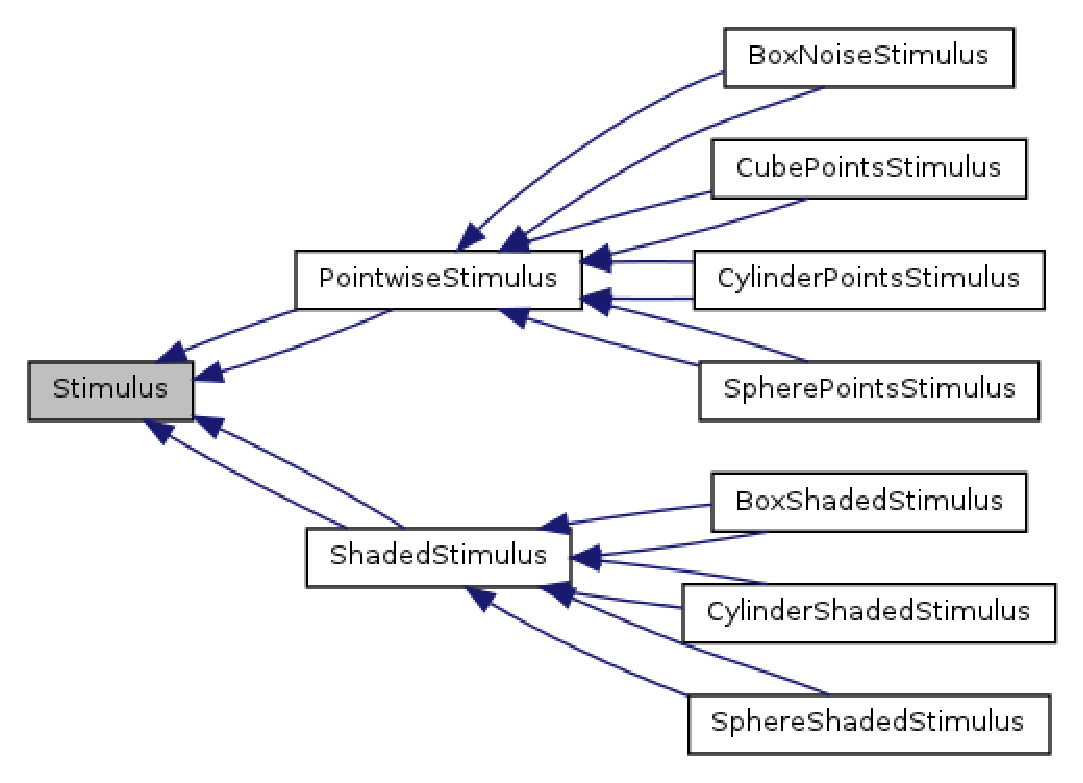
\includegraphics[width=0.8\textwidth]{inheritGraphStimuli.eps}
% \caption{Inheritance scheme of visual stimuli abstraction.}
% \label{fig:stimulusscheme}
%\end{figure}
%
%Common member variables of the point-wise stimulus inherited classes are two
%array of points, the points composing the stimulus itself and another array,
%called \verb=specialPoints= that contains a special set
%of points, varying for every stimulus, for example a cubic stimulus has $8$
%special points representing its vertexes, a spherical stimulus has $n+1$ special
%points: its center and other $n$ points on the 
%sphere surface and so on. These points are treated by \verb=StimulusDrawer=
%differently and enables the experimenter to visualize stimulus characteristics.
%
%Finally for the rendering of the visual stimuli a class
%\label{sec:stimulusdrawer} \verb=StimulusDrawer= is available. It uses
%prebuffered display lists to create fast visualization of fixed stimuli and also
%has options for special points visualization.

\subsection{Communication}
Communication module advocates the handling of what copes with PC external
hardware interfaces.
\paragraph{Serial port interface and Velmex motors}
A generic but thin wrapper written around the \verb=Boost::asio= which exploit C++ stream
is provided.
The wrapper, \verb=SerialStream= allows the user to treat the serial port as a
usual C++ stream thanks to the overloading of the stream insertion operator
\verb=<<= but also to handle more advanced features, such as baud rate and
parity bit settings.

Functions for the movement of Velmex motors are provided in a dedicate namespace because varying on the experimental setup, they can change very much.
They are written completely ignoring the proprietary drivers by writing apposite strings via the before mentioned \verb=SerialStream= wrapper.
All these functions for the movements of objects in the experimental setup are provided both in their blocking and asynchronous flavors.
Non blocking functions allows to move the motors while keeping the experiment running.
\paragraph{Eyegaze data retrieval}
XXX


\section{Calibration of an active vision system}
\subsection{Rigid-body transformation estimation}\label{sec:rigidbodytransformationestimation}
In the following sections we will use $\mathbb{E}^3$ to denote the familiar
three-dimensional Euclidean space\footnote{We will denote common three-dimensional vectors with lowercase bold letters $(\mathbf{x}, \mathbf{p})$, unit-norm three dimensional vectors with lowercase bold letters and a hat: $\mathbf{\hat{u}},\mathbf{\hat{v}}$,  
matrices with uppercase bold letters $(\mathbf{A}, \mathbf{B})$, identity matrix with $\mathbf{I}$, scalars with lowercase letters $a,b,c$. We will use the same convention for points and vectors whenever their correct dimensions is clear from the context.}: every point $\mathbf{x} \in \mathbb{E}^3$ can
be identified with a point in $\mathbb{R}^3$ with three coordinates
$$\mathbf{x} = [x_1, x_2,x_3]^T$$

In order to describe the rigid-body motion one should in
principle specify the trajectory of every single point on the object but
fortunately for rigid objects we do not need to specify the
motion of every point, it's sufficient to specify the motion of one and the
motion of three coordinate axes attached to that point, because the distance
between any points on it does not change over time as the object moves.

This rigid-body motion can be described at every temporal instant by a $3\times
3$ rotation matrix $\mathbf{R} \in \mathbb{R}^{3\times 3}$ and a displacement
vector $\mathbf{t} \in \mathbb{R}^{3}$ such that for a point $\mathbf{x}_i$ on
the object we have:
\begin{equation}\label{eq:affinemotion}
  \mathbf{x}_i(t) = \mathbf{R}(t)\cdot \mathbf{x}_i(t_0) + \mathbf{t}(t)
\end{equation}
%The previous equation can be modified to include also a scaling factor $c$, but we don't need it since we are working with rigid-body transformation.

We note that the coordinates transformation for a full rigid body motion is not
linear but \emph{affine}, nonetheless we may convert such an 
affine transformation to a linear one by using homogeneous coordinates appending
$'1'$ to the coordinates of a point $\mathbf{x} \in \mathbb{E}^3$ yielding
a vector  in $\mathbb{R}^4$. Using the $4$ dimensional notation, we can rewrite (\ref{eq:affinemotion}) in a linear fashion

\begin{align}\label{eq:homogenized}
\mathbf{H} = \begin{bmatrix} \mathbf{R} & \mathbf{t} \\ \mathbf{0} & 1
\end{bmatrix}
\end{align}
The matrix $\mathbf{H}\in \mathbb{R}^{4\times 4}$ is called the
\emph{homogeneous representation} of the rigid-body motion. This allows us 
to represent rigid-body motion as linear column vector-matrix multiplication and is very useful in recovering the coordinates of a point as seen from another reference frame, which transformation relative to the original is described by $\mathbf{H}$.

It's possible to estimate the transformation parameters $\mathbf{R}$ and
$\mathbf{t}$ between two sets of points for which corresponding pairs have been determined. This is called the \emph{absolute orientation problem} and is accomplished by the a class of algorithms called \emph{point fitting algorithms}. We use \emph{Umeyama}'s method \cite{umeyama}, the most reliable and stable. 

Due to its ubiquity, in the next sections we'll refer to the Umeyama algorithm as that function with input the two set of points (source and destination) and as output the \emph{rigid-body motion matrix} $\mathbf{H}$:
\begin{equation}
 \mathbf{H} = \textrm{umeyama}\left( \mathbb{X}_{\textrm{src}}, \mathbb{X}_{\textrm{dst}} \right)
\end{equation}

Umeyama method estimates both $\mathbf{R}$ and $\mathbf{t}$ (and an
additional scaling parameter $c$) by minimizing a least-square cost function.
\begin{equation}\label{eq:umeyama}
 \dfrac{1}{N}  \sum \limits_{i=0}^N \begin{Vmatrix} \mathbf{x}_{i}(t_0)
-c(\mathbf{R} \cdot \mathbf{x}_i(t) +\mathbf{t}) \end{Vmatrix}^2
\end{equation}
where in our case we set the number of destination and source points $N=3$ and
$c=1$. The algorithm is based on the singular value
decomposition (SVD) of the covariance matrix $\Sigma \in
\mathbb{R}^{d \times d}$ of the input point sets, where $d$ is corresponding to the dimension of the space $d=3$ \cite{umeyama,DBLP:books/daglib/0086372,eigenweb}. 

In this following analysis $\mathbf{H}$ we'll represent the 3-D rigid transformation from \emph{source} to \emph{destination} points directly as matrix-column vector multiplication:
\begin{equation}
 \mathbf{x}_i(t) =  \mathbf{H}(t)\cdot \mathbf{x}_i(t_0) = \begin{bmatrix} \mathbf{R} & \mathbf{t} \\ 0 & 1\end{bmatrix} \begin{bmatrix} \mathbf{x}_i(t_0) \\ 1\end{bmatrix}\qquad \forall
i=1,\ldots,N
\end{equation}
clearly supposing that $\mathbf{x}_i(t_0)$ and $\mathbf{x}_i(t)$ are homogenized by adding a $1$ as fourth row.

\subsection{Ghost points estimation}

\emph{Ghost points} are here referred as those points in the VE without a
physical counterpart (basically a physical marker representing it), but which
are computed from another set of point (reference). They will always be denoted
 with a tilde, e.g. $\tilde{\mathbf{x}}$

A \emph{ghost point} is a central concept, because it give more degrees of
freedom to the user, allowing him to move freely in the space, without bothering
about physical markers occlusion due to obstacles in the optic path from the
camera to the emitting diode\footnote{We call a marker in the optical range of the tracking system a \emph{visible} marker, \emph{non-visible} otherwise}.
They can be estimated given a relation with at
least three reference points. For each of the ghost points, an affine
transformation of the form in eq.(\ref{eq:homogenized}) must be computed via an
\emph{absolute orientation algorithm} such as \emph{Umeyama}.

Let's fix a rigid-body and attach to it two set of markers, the first acting as
\emph{reference}: $\mathbb{X}_{\textrm{ref}} = \{
\mathbf{x}_1,\mathbf{x}_2,\mathbf{x}_3 \}$,
and the second $\mathbb{X}_{\textrm{image}} =\{ \mathbf{x}_i \}$  $i=4,\ldots,N$
as the initial images of the ghost points $\mathbf{\tilde{x}}_{i}$  which will
undergo the rigid-body transformation $\mathbf{H}$.

As discussed earlier, because of rigid-body condition, both the sets of points $\mathbb{X}_{\textrm{ref}}$ and $\mathbb{X}_{\textrm{image}}$ will undergo the same rigid-body motion 
transformation $\mathbf{H}$ so 
that the physical relative distance of points inside the reference set
$\mathbb{X}_{\textrm{ref}}$ are fixed $\forall t>t_0$: otherwise the
algorithm will produce inconsistent results (rigid-body motion assumption fails).

The ghost points  $\tilde{\mathbf{x}}_i(t)$ relative to their previous images
$\mathbf{x}_i(t_0) \in \mathbb{X}_{\textrm{image}}$ are then calculated when the motion parameters matrix
$\mathbf{H}$ is extracted by applying the absolute orientation problem to the
two sets of reference points $\mathbb{X}_{\textrm{ref}}(t_0)$ and $\mathbb{X}_{\textrm{ref}}(t)$ and then obtaining:
\begin{equation}
	\tilde{\mathbf{x}}_i(t) = \mathbf{H}(t)\cdot \mathbf{x}_i(t_0) \quad
\forall i=4,\ldots,N
\end{equation}

The \verb=CoordinatesExtractor= class comes in help both in head movement matrix
estimation, in ghost finger retrieval and generally where the experimenter has
to estimate ghost points.

An example of usage of a \emph{ghost points} estimation method is the one to
find eyes position only by wearing a patch with three reference points
$\mathbb{X}_{\textrm{ref}}$ and a
pair of glasses with two markers on the opposite sides, forming the set
$\mathbb{X}_{\textrm{image}}= \{ \mathbf{x}_4, \mathbf{x}_5 \}$.
 
First a shot of the two set of points is taken. The set $\mathbb{X}_2$ is needed
to estimate the eyes positions: because $\mathbf{x}_4$ and $\mathbf{x}_5$ are
chosen to lie
along the line through left and right eye, their position can simply be computed
as:
\begin{eqnarray*}
\tilde{\mathbf{x}}_{er}(t_0) =  \frac{\mathbf{x}_4(t_0) + \mathbf{x}_5(t_0)}{2}
-  \frac{ (\mathbf{x}_4(t_0) - \mathbf{x}_5(t_0)) }{||\mathbf{x}_4(t_0) -
\mathbf{x}_5(t_0))||}\frac{\textrm{IOD}}{2} \\
\tilde{\mathbf{x}}_{el}(t_0) =  \frac{\mathbf{x}_4(t_0) + \mathbf{x}_5(t_0)}{2}
+  \frac{ (\mathbf{x}_4(t_0) - \mathbf{x}_5(t_0)) }{||\mathbf{x}_4(t_0) -
\mathbf{x}_5(t_0))||}\frac{\textrm{IOD}}{2}
\end{eqnarray*}

where $\textrm{IOD}$ is the \emph{interocular distance} parameter.

The two eye position for the following frames $t>t_0$ are then simply updated
once $\mathbf{H}$ is known:
\begin{eqnarray*}
	\mathbf{x}_{er}(t) &= \mathbf{H} \cdot \mathbf{x}_{er}(t_0) \\
	\mathbf{x}_{er}(t) &= \mathbf{H} \cdot \mathbf{x}_{er}(t_0) 
\end{eqnarray*}

An algorithmic overview of the eye position estimation method is given (alg. \ref{alg:eyepositionestimation}).
\begin{algorithm}[htb]\label{alg:eyepositionestimation}
\SetAlgoCaptionLayout{textbf}
\KwIn{$\mathbb{X}_{\textrm{ref}} = \{
\mathbf{x}_1(t_0),\mathbf{x}_2(t_0),\mathbf{x}_3(t_0) \}$,
$\mathbb{X}_{\textrm{image}}=\{ \mathbf{x}_4(t_0) , \mathbf{x}_5(t_0) \}$,
$\textrm{IOD}$
}
\KwOut{$\mathbf{x}_{er}$,$\mathbf{x}_{el}$}

\tcc{Compute the eye position at first time frame $t_0$ given their interocular
distance (IOD)} 

\While{ $\mathbf{x}_4$ and $\mathbf{x}_5$ are visible }
{
\begin{equation*}
\mathbf{x}_{er}(t_0) =  \frac{\mathbf{x}_4(t_0) + \mathbf{x}_5(t_0)}{2} - 
\frac{ (\mathbf{x}_4(t_0) - \mathbf{x}_5(t_0)) }{||\mathbf{x}_4(t_0) -
\mathbf{x}_5(t_0))||}\frac{\textrm{IOD}}{2}
\end{equation*}

\begin{equation*}
\mathbf{x}_{r}(t_0) =  \frac{\mathbf{x}_4(t_0) + \mathbf{x}_5(t_0)}{2} +  \frac{
(\mathbf{x}_4(t_0) - \mathbf{x}_5(t_0)) }{||\mathbf{x}_4(t_0) -
\mathbf{x}_5(t_0))||}\frac{\textrm{IOD}}{2}
\end{equation*}
}
\tcc{Update eyes position} 
\For{ $t>t_0$ }
{
\begin{equation*}
\mathbf{H} = \textrm{umeyama}\left( \mathbb{X}_{\textrm{ref}}(t_0),
\mathbb{X}_{\textrm{ref}}(t) \right) 
\end{equation*}

\begin{eqnarray*}
\mathbf{x}_{er}(t) & = \mathbf{H} \cdot \mathbf{x}_{er}(t_0) \\
\mathbf{x}_{el}(t) &= \mathbf{H}  \cdot \mathbf{x}_{er}(t_0)
\end{eqnarray*}

}
\caption{Eye position estimation algorithm}
\end{algorithm}

When applied to eye position estimation, $\mathbf{H}$ represent the \emph{head motion
matrix} and is composed by a rotational and a translational part, both relative to the last calibration, and in general not to the global frame but with respect the last defined frame.
We'll address the way to make the rotational and translation part of $\mathbf{H}$ relative to a global and consistent coordinate frame at paragraph \ref{sec:consistentcalibration}.

Three angles can be extracted from the rotation part of $\mathbf{H}$, once a
convention is chosen.
They are the Euler angles of the rotation $\psi, \theta, \phi$, we have chosen
the \emph{yaw-pitch-roll} convention: 
\emph{yaw} is the angle when moving the head left to right (rotation around
$\mathbf{\hat{y}}$-axis), \emph{pitch} is up and down (rotation around
$\mathbf{\hat{x}}'$-axis) and
roll, which we usually don't experience (but is important) is when you tilt your head (rotation
around $\mathbf{\hat{z}}''$-axis)
\footnote{We use the colon notation appositely to point out that the transformed axes are not the global reference frame axes: $\mathbf{\hat{x}}' \neq \mathbf{\hat{x}}$ and  $\mathbf{\hat{z}}'' \neq \mathbf{\hat{z}}'  \neq \mathbf{\hat{z}}$ }
It should be pointed out here that the
order of Euler angles is important and not 
interchangeable (basically because of non commutativity of matrix-matrix
product).

\subsection{Consistent calibration}\label{sec:consistentcalibration}
Some reader could have noted that here we are speaking only about relative
transformation between set of points or reference frames.

How to perform a calibration that allows us to extract rotation angles
consistently w.r.t. a global
reference frame $O_{xyz}$ and not with respect to the  latest defined  set $\mathbb{X}_{\textrm{ref}}$?

Two alignment must be accomplished: \emph{orientation} and \emph{translation} alignment.
After the two alignments are done with a predefined tolerance error $\epsilon$, the $\mathbb{X}_{\textrm{ref}}$ can be redefined and since that instant rotations and translations will be 
relative to the origin.

The orientation alignment is  performed by aligning the \emph{gaze direction} vector to the global
reference frame depth axis $\mathbf{\hat{z}}$. We must here specify that gaze direction is only dependent on head rotation and not on ocular movements.

The gaze direction is a normalized vector $\mathbf{\hat{u}} \in \mathbb{R}^3$ and can be computed
as
\begin{equation}\label{eq:gazedirection}
 \mathbf{\hat{u}}(t) = \mathbf{R}(t) \cdot [ 0,0,-1]^T
\end{equation}

The intersection point $\mathbf{u}^{*}$ of the line passing through $\mathbf{x}_{er}$ and $\mathbf{x}_{er}+\hat{\mathbf{u}}$ with a $xy$ plane at some $z$ is computed by mean of line-plane intersection.

\begin{equation}\label{eq:gazedirectionintersection}
      \mathbf{u}^{*} = \frac{(\mathbf{p}_0-\mathbf{u}_0) \cdot \mathbf{\hat{n}}}{\mathbf{\hat{u}}\cdot \hat{\mathbf{n}}} \mathbf{\hat{u}} + \mathbf{x}_{er}
\end{equation}


The full alignment is performed by aligning both the orthographic projection of right eye $\proj_{\mathbf{\hat{n}}} ({\mathbf{x}_{er} }) =  [ x_{er_x}, x_{er_y}, z ]^T$ and $\mathbf{u}^{*}$ 
to a central point with coordinates $\mathbf{x}_{\textrm{center}}=\left[ 0,0,z\right]^T$.

\begin{algorithm}[htb]\label{alg:consistentcalibration}
\SetAlgoCaptionLayout{textbf}
\KwIn{$\mathbb{X}_{\textrm{ref}}(t_1) = \{
\mathbf{x}_1(t_1),\mathbf{x}_2(t_1),\mathbf{x}_3(t_1) \}$,
$\mathbb{X}_{\textrm{ref}}(t) = \{
\mathbf{x}_1(t),\mathbf{x}_2(t),\mathbf{x}_3(t) \}$, tolerance radius $\epsilon =2 \textrm{ mm}$ }
\For{ $t>t_1$ }
{
\While{ $|| \proj_{\mathbf{\hat{n}}}({\mathbf{x}_{er} }) - \mathbf{x}_{\textrm{center}} || > \epsilon$ and  $||
\mathbf{u}^{*} - \mathbf{x}_{\textrm{center}}) || > \epsilon$ }
{
$
\mathbf{H} = \textrm{umeyama}\left( \mathbb{X}_{\textrm{ref}}(t_1),
\mathbb{X}_{\textrm{ref}}(t) \right)
$\;
Compute the line-of-sight direction $\mathbf{\hat{u}}$   \;
Compute intersection of gaze direction on plane  $\mathbf{u}^{*}$  \;
Compute the right eye orthographic projection $\proj_{\mathbf{\hat{n}}} ({\mathbf{x}_{er} })$   \;
}
}
\caption{Consistent calibration}
\end{algorithm}

Algorithm \ref{alg:consistentcalibration} ensures that the rotational part of $\mathbf{R}\equiv \mathbf{I}$ when the head orientation is the same of the global reference frame.
This is clearly an advantage with respect to other methods: first the user doesn't need to cope with Euler angles, second everything is performed numerically, without the slow and error-prone
phase of manually write complex $\sin()$ and $\cos()$ formulas. The precision of the orientation is then dependent on a simply controllable tolerance radius $tol$ which is the radius of the
circle in which both $\proj_{\mathbf{\hat{n}}}({\mathbf{x}_{er} })$ and $\mathbf{u}^{*}$ should stay to produce a correct and consistent orientation.

This is the only method that guarantees a 6 DOF consistent calibration of a observer in active vision experiments.

For a viewer at $500$ mm from the projection plane and a tolerance radius $\epsilon = 2$ mm we get an orientation error in pitch and yaw of $\Delta \theta = \arctan ( \epsilon/(2z) \approx 10^{-4} $ degrees.
and a translation error of $\Delta \leq \epsilon$ both in $x$ and $y$ translations.

A correct orientation around the $\hat{\mathbf{z}}$ axis (roll component) should be addressed by showing to the subject the line through the two orthographic projection of left and eye right and
 making it parallel to the ground, basically checking that $|\proj_{\mathbf{\hat{n}}}({\mathbf{x}_{er} })_y - \proj_{\mathbf{\hat{n}}}({\mathbf{x}_{el} }_y)|> \epsilon$. Since this task is generally difficult for the non experienced user and because typically the roll of the head at rest is very low, this alignment can be usually ignored.

Once the consistent calibration described here is done, the visual psychophysics experiment can start.
% \subsection{Markers velocities estimation and filtering}
% \label{sec:optotrakvelocities}
% We adopted a backward finite difference for the estimation of the velocity: for
% the $k$-th marker we compute the velocity $\mathbf{v}$ at discrete time frame
% $t$ given its current and two previous positions $\mathbf{x}_{t}$,
% $\mathbf{x}_{t-1}$, $\mathbf{x}_{t-2}$ 
% as follows:
% \begin{equation}
%  \mathbf{v}_{k} = \dfrac{ 3\mathbf{x}_t - 4\mathbf{x}_{t-1} + \mathbf{x}_{t-2}
% }{2 \Delta t }
% \label{eq:velocityestimation}
% \end{equation}
% The time interval $\Delta t$ is computed through system calls to high-resolution
% operative-system-dependent function (and not using C provided \verb=clock()=
% function which is very inaccurate).
% Windows provides \verb=QueryPerformanceCounter()= function, and Unix, Linux and
% Mac OS X systems have the \verb=gettimeofday()=  command, which is declared in
% \verb=sys/time.h=.
% Both functions can measure at least 1 micro-second
% difference\footnote{\url{http://www.songho.ca/misc/timer/timer.html}}. 
% 
% The smoothing of estimated velocities (\ref{eq:velocityestimation}) is made
% through a real-time digital infinite impulse response (IIR) single pole filter.
% The processed output takes then the form:
% \begin{equation}
%  \mathbf{v}_{t} \leftarrow A \mathbf{v}_{t} + (1-A)\mathbf{v}_{t-1}
% \end{equation}
% where the gain $A=0.3 $ is a good compromise between noise filtering
% characteristics and phase delay of response. The cutoff frequency for such a
% filter is $XXX$.
% 
% \subsection{Velocity transformations}
% Velocities are only available for physical markers, but sometimes we need to get them also for \emph{ghost points}.
% Again, the concept of rigid-body motion matrix comes in help.
% 
% Let us suppose that a \emph{ghost point} is computed as follows:
% \begin{equation*}
%  \mathbf{\tilde{x} }(t) = \mathbf{H}(t) \cdot \mathbf{x}(t_0)
% \end{equation*}
% Then the velocity of the point $\mathbf{\tilde{x}}$ relative to the instantaneous reference frame is
% \begin{equation*}
%  \mathbf{\dot{\tilde{x}}}(t) = \mathbf{\dot{H}} \cdot \mathbf{x}(t_0)
% \end{equation*}
% 
% In order to express $\mathbf{\dot{\tilde{x}}}(t)$ in terms of components in the moving frame, we substitute $\mathbf{x}(t_0)$ by $\mathbf{H}^{-1}(t)\cdot \mathbf{{\tilde{x}}}(t)$ so that:
% \begin{equation}
%  \mathbf{\dot{\tilde{x}}}(t) =  \mathbf{\dot{H}}(t)\cdot \mathbf{H}^{-1}(t)\cdot \mathbf{{\tilde{x}}}(t) 
% \end{equation}
% 
% % For example, suppose that a viewer is in another coordinate frame displaced relative to the main frame by a rigid-body transformation $\mathbf{G}$. Then the coordinates of the same point $\mathbf{x}$ 
% % relative to this frame are $\mathbf{y}(t) = \mathbf{G} \mathbf{x}(t)$. We compute the velocity in the new frame and obtain
% % \begin{equation}
% %  \mathbf{\dot{y}}(t) = \mathbf{G}\cdot \mathbf{H}(t) \cdot \mathbf{H}^{-1}(t)\cdot \mathbf{G}^{-1} \mathbf{y}(t)
% % \end{equation}
% % 
% Now note that\footnote{Remember that a rotation matrix is always
% orthogonal
%  i.e.
% $\mathbf{R}^{-1}_{(\mathbf{u},\theta)}=\mathbf{R}^T_{(\mathbf{u},\theta)}$.  }
% \begin{equation*}
% \mathbf{\dot{H}} \cdot \mathbf{H}^{-1} := \begin{bmatrix}\mathbf{\dot{R}} \cdot \mathbf{R}^T(t) &\quad \mathbf{\dot{t}}(t) -\mathbf{\dot{R}}(t) \mathbf{R}^T(t) \mathbf{t}(t)\\ \mathbf{0} & 0\end{bmatrix}.
% \end{equation*}
% 
% Call $\boldsymbol \Omega(t) = \mathbf{\dot{R}} \cdot \mathbf{R}^T$ \emph{angular velocity tensor} and 
% $$\mathbf{v}(t) = \mathbf{\dot{t}}(t) -\mathbf{\dot{R}}(t) \mathbf{R}^T(t) \mathbf{t}(t)$$
% the translational velocity vector.
% 
% This lead us to write
% \begin{equation*}
% \mathbf{\dot{H}} \cdot \mathbf{H}^{-1} := \begin{bmatrix}\boldsymbol \Omega(t) & \mathbf{v}(t) \\ \mathbf{0} & 0\end{bmatrix}
% \end{equation*}
% A $4 \times 4$ matrix of this form is also called a \emph{twist}.
% 
% 
% One can show that it holds \cite{Ma:2003:IVI:971144}:
% \begin{equation}\label{eq:angularvelocitytensor}
% \boldsymbol \Omega(t) = \mathbf{\dot{R}}\cdot\mathbf{R}^T = \begin{pmatrix} 0 & -\omega_z(t) & \omega_y(t) \\ \omega_z(t) & 0 & -\omega_x(t) \\ -\omega_y(t) & \omega_x(t) & 0 \\ \end{pmatrix}
% \end{equation}
% 
% where $\omega_x, \omega_y, \omega_z$ are the components of the usual angular velocity (pseudo)vector $\boldsymbol \omega \in \mathbb{R}^3$: the angular velocity tensor act as if it were a  $\boldsymbol \omega(t) \times $ operator.
% 
% Now we are ready to compute the term $\mathbf{\dot{R}}$, from (\ref{eq:angularvelocitytensor}) we obtain:
% \begin{equation*}
%  \mathbf{\dot{R}} = \boldsymbol \Omega(t) \cdot \mathbf{R}(t)
% \end{equation*}
% 
% Angular velocity vector (and then tensor) can be obtained from rotation matrices via the so called \emph{axis-angle} representation.
% Let's define $\mathbf{Y}=\mathbf{R}(t) \mathbf{R}^{T}(t+\Delta t)$\footnote{Remember $(\mathbf{A} \cdot \mathbf{B})^{-1} = \mathbf{B}^{-1} \mathbf{A}^{-1}$ } as the rotation matrix that rotates the body from the position at time $t$ to the position at time $t+\Delta t$.
% This is a rotation around the axis along $\boldsymbol \omega$ through the angle $|\boldsymbol \omega| \Delta t$. 
% 
% Angle and axis are obtained as:
% \begin{eqnarray}\label{eq:axisanglerepresentation}
% \theta = \arccos &\left( \dfrac{\tr(\mathbf{Y}(t)) - 1}{2}\right) \nonumber \\
% \boldsymbol \omega = \dfrac{1}{2 \sin(\theta)} &\begin{bmatrix} \mathbf{Y}_{3,2}(t)-\mathbf{Y}_{2,3}(t) \\ \mathbf{Y}_{1,3}(t)-\mathbf{Y}_{3,1}(t) \\ \mathbf{Y}_{2,1}(t)-\mathbf{Y}_{1,2}(t) \end{bmatrix} 
% \end{eqnarray}
% The last equation allows us to compute the angular velocity tensor as in (\ref{eq:angularvelocitytensor}) and therefore we can compute velocity transformation between two reference frames as:
% 
% \begin{equation*}
%  \mathbf{\dot{\tilde{x}}}(t) = \boldsymbol \Omega(t) \cdot \mathbf{\tilde{x}}(t) + \mathbf{v}(t)
% \end{equation*}
% When referring to the original known points $\mathbf{x}(t_0)$ for which ghost the point $\mathbf{\tilde{x}}$ is computed then the last equation is:
% \begin{equation}\label{eq:ghostpointvelocityestimation}
%  \mathbf{\dot{\tilde{x}}}(t) = \boldsymbol \Omega(t) \cdot \mathbf{H} \cdot \mathbf{x}(t_0) + \mathbf{v}(t)
% \end{equation}
% 
% Equation (\ref{eq:ghostpointvelocityestimation}) is the basis formula in estimation of non physical points and is used extensively in CNCSVision.
% 
% We can extend eq. (\ref{eq:ghostpointvelocityestimation}) to evaluate the velocity of a ghost point as seen from another reference frame whose coordinate transformation from the global frame is $\mathbf{G}=[\mathbf{R}_G, \mathbf{t}_G ]$.
% We obtain:
% \begin{equation}
%  \mathbf{\dot{\tilde{x}}}_{\mathbf{G}} = \mathbf{G}(t)^{-1}\cdot \mathbf{\dot{H}}(t) \cdot \mathbf{H}(t)^{-1} \cdot \mathbf{G}(t)\cdot \mathbf{{\tilde{x}}}=\mathbf{G}(t)^{-1}\cdot \mathbf{\dot{H}}(t) \cdot \mathbf{H}(t)^{-1} \cdot \mathbf{G}(t)\cdot \mathbf{H} \mathbf{x}(t_0)
% \end{equation}
% 
% % 
% % Angular velocity tensor can also be computed by mean of the logarithm map: suppose $\mathbf{R}(t)$ and $\mathbf{R}(t+dt)$ be two rotation matrices, then 
% % \begin{equation}
% %  \mathbf{R}(t+dt) = e^{ \boldsymbol \Omega dt} \mathbf{R}(t)
% % \end{equation}
% % this means that
% % \begin{equation}
% %  \log\left(\mathbf{R}(t) \mathbf{R}^{-1}(t+dt) \right) = \boldsymbol \Omega(t) dt
% % \end{equation}
% % so
% % \begin{equation}
% %  \boldsymbol \Omega(t) = \dfrac{ \log\left(\mathbf{R}(t) \mathbf{R}^{-1}(t+dt) \right)}{dt} \approx \frac{1}{dt} \left( \mathbf{Y} - \frac{\mathbf{Y}^2}{2} + \frac{\mathbf{Y}^3}{3} - \frac{\mathbf{Y}^4}{4} + \ldots \right )
% % \end{equation}
% % where we defined $\boldsymbol Y = \mathbf{R}(t) \mathbf{R}^{-1}(t+dt) -\mathbf{I} $ and approximated matrix logarithm with its Taylor expansion.


\subsection{Generalized perspective projection}\label{sec:generalizedperspectiveprojection}
Most OpenGL applications select a FOV (field of view), specify near and 
far clipping plane distances and call \verb=gluPerspective=, they implicitly
assume the user is located directly in front of the screen facing perpendicular
to it and looking toward its center or at least a 
perspective rooted at the origin and a projection screen on the XY plane. These
assumptions don't hold in the \emph{VE} circumstances, because \emph{VE}
introduces first-person motion tracking perspective, 
stereoscopic viewing and arbitrarily oriented displays.

As is common in \emph{VE} systems a motion tracking system senses the position
of the eyes and the orientation of the head in 
order to allow the 3D spatial positions of each of his eyes to be computed
relative to position of the display. Now because the subject is free to move,
the view positions does not remain centered upon any 
of the screens and the \verb=gluPerspective= function fails. Additionally when
the display doesn't lie in the XY plane, the \verb=glFrustum= function fails.

CNCSVision implements the generalized perspective projection for both active and
passive viewing in the most generic way. We follow the implementation given in
\cite{kooima}. Note that this method permits
also to implement a correct stereoscopic display.

Let us fix a global reference frame $O_{xyz}$ and define three points
$\mathbf{p}_{a}$, $\mathbf{p}_b$, $\mathbf{p}_c$ lying on the lower left, lower
right and upper left corners of the rectangular projection area 
(can be a PC-monitor display area, a LED wall or anything else). These points
are used to compute an orthonormal basis $\mathbf{v}_r$,
$\mathbf{v}_u$,$\mathbf{v}_n$ for the screen space\footnote{Loosely speaking,
the unit vectors of the screen space orthonormal basis give us a basis for
describing points relative to the screen.}:
\begin{eqnarray}
 \mathbf{v}_r = \frac{\mathbf{p}_b-\mathbf{p}_a}{||\mathbf{p}_b-\mathbf{p}_a||}
\nonumber \\
 \mathbf{v}_u = \frac{\mathbf{p}_c-\mathbf{p}_a}{||\mathbf{p}_c-\mathbf{p}_a||}
\nonumber \\
 \mathbf{v}_r = \frac{\mathbf{v}_r \times \mathbf{v}_u}{||\mathbf{v}_r \times
\mathbf{v}_u||}
\end{eqnarray}


Let us start considering the position of the observer (projection center, or
camera or eye) relatively to the screen and call it $\mathbf{p}_e$. 
Here we want to allow the eye to move freely but have in every case the correct
perspective computed, this is where \verb=glFrustum(...)= comes in. As
documented, this function takes parameters giving the left,
right, bottom, and top \emph{view frustum} extents: $l,r,t,b$.

 \begin{figure}[ht]
 \centering
 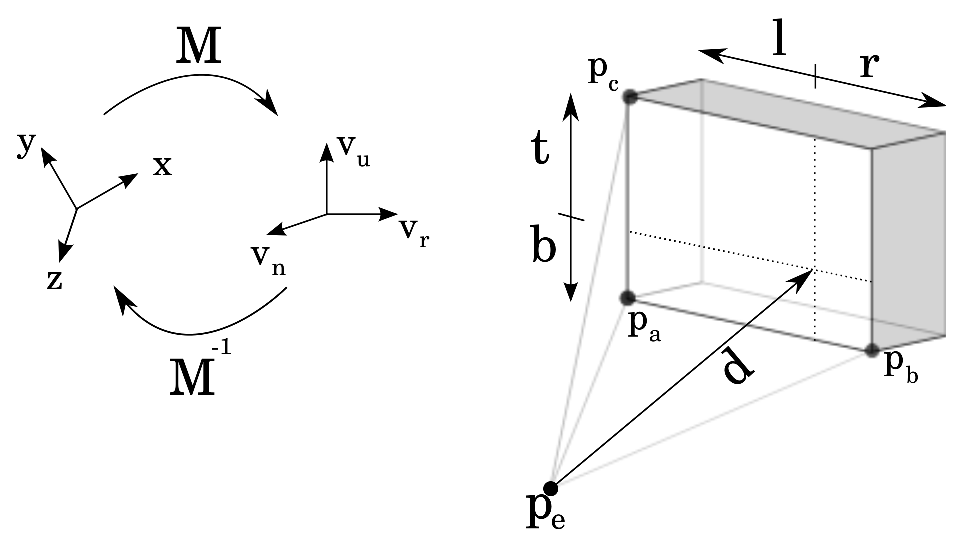
\includegraphics[width=0.6\textwidth]{genperspectiveprojection2.eps}
 % perspectiveprojection.ps: 596x842 pixel, 72dpi, 21.03x29.70 cm, bb=0 0 596 842
 \caption{Generalized perspective projection scheme with meaning of each
variable.}
 \label{fig:perspectiveprojection}
\end{figure}


The value for $l,r,t,b$ are extracted from the previous computed quantities, in
particular, let $d$ be the distance from the eye to the screen surface, then:
\begin{equation}
 d = - \mathbf{v}_n \cdot ( \mathbf{p}_a -\mathbf{p}_e )
\end{equation}

Because frustum extents are specified at near plane $n$, using triangle
similarity arguments, we obtain

\begin{eqnarray}
& l = (\mathbf{v}_r \cdot \mathbf{v}_a ) n /d &\hspace{6mm} r = (\mathbf{v}_r
\cdot \mathbf{v}_b ) n /d \nonumber \\
& b = (\mathbf{v}_u \cdot \mathbf{v}_a ) n /d &\hspace{6mm} t = (\mathbf{v}_r
\cdot \mathbf{v}_c ) n /d 
\end{eqnarray}
where $\mathbf{v}_{\{a,b,c\}} = \mathbf{p}_{\{a,b,c\}}-\mathbf{p}_e$.

We form the \emph{OpenGL} perspective projection matrix $\mathbf{P}$ then as
follows:
\begin{align*}
\mathbf{P}= \begin{bmatrix}
\frac{2n}{r-l} & 0 & \frac{r+l}{r-l} & 0 \\ 
0 & \frac{2n}{t-b} & \frac{t+b}{t-b} & 0 \\ 
0 & 0 & -\frac{f+n}{f-n} & -\frac{2fn}{f-n} \\ 
0 & 0 & -1 & 0 
\end{bmatrix}
\end{align*}

The matrix $\mathbf{P}$ now represent a frustum lying with the front plane on
the $XY$ plane: in order to allow a general treatise of the screen as projection
surface (and then distinguish between \emph{active} and \emph{passive} display) we must define a transformation matrix which 
accounts both for the rotation and for the translations relative to the canonical base in the reference
frame $O_{xyz}$ origin.

Let's call $\mathbf{M}$ this $4 \times 4$ matrix (an \emph{homogenized} 3D
rotation matrix $\mathbf{R}_M$):

\begin{align*}
\mathbf{M} =
\begin{bmatrix}
v_{rx} & v_{ux} & v_{nx} & 0 \\
v_{ry} & v_{uy} & v_{ny} & 0 \\
v_{rz} & v_{uz} & v_{nz} & 0 \\
0 & 0 & 0 & 1
\end{bmatrix}
=
\begin{bmatrix}
\mathbf{R}_M & 0 \\
\mathbf{0} & 1 
\end{bmatrix}
\end{align*}

Recall that in OpenGL when we want to rotate our frustum to align it within our
tracker space we instead rotate our tracker space to align it with our frustum.
With this in mind, the right matrix to apply 
to $\mathbf{P}$ is the inverse (or transposed) of $\mathbf{M}$.

A last point in the creation of the generalized perspective projection matrix is
the eye position. Remember also in this case if we want to move our eye to the
left, we must instead
move the world to the right and vice-versa. This can be accomplished with a last
multiplication by a $4 \times 4$ translation matrix $\mathbf{T}$:

\begin{align*}
\mathbf{T} =
\begin{bmatrix}
1 & 0 & 0 & -p_{e_x} \\
0 & 1 & 0 & -p_{e_y} \\
0 & 0 & 1 & -p_{e_z} \\
0 & 0 & 0 & 1 
\end{bmatrix}
\end{align*}

Finally the generalized perspective matrix to be used in a active vision
experiment with head tracking is the following

\begin{equation}
\mathbf{P'} = \mathbf{P} \cdot \mathbf{M}^T \cdot \mathbf{T}
\end{equation}

Within the \emph{Eigen} framework the matrix multiplication is a fully
vectorized and optimized operation, so we choose to keep it on CPU in order to have
more mathematically clear code and 
to disentangle visualization from computation.

In an active vision experiment we distinguish 
between \emph{active} and \emph{passive display}.

An \emph{active view display}, is one in which the observer moves freely in the
\emph{VE} and for which perspective projection is
computed with $\mathbf{M} = \mathbf{I}_{4\times 4}$, because the screen surface
normal is parallel to the depth direction and the screen corners are \emph{fixed} in
the global reference frame $O_{xyz}$ .

A \emph{passive view display}, is instead the one in which the projection
surface moves virtually ``attached'' to the head with the normal always parallel
to the gaze direction.

This kind of view display can be simply obtained within this framework by
transforming the screen corners with the \emph{head transformation matrix}
$\mathbf{H}$ and applying what described before for the new screen corners
$\mathbf{\tilde{p}}_{\{a,b,c \}}$
\begin{eqnarray}
\mathbf{\tilde{p}}(t)_{\{a,b,c\}} = \mathbf{H}(t) \mathbf{p}_{\{a,b,c\}}
\end{eqnarray}

% 
% \subsubsection{Technical issues for a stereoscopic display}
% While the stereoscopic vision is simply achieved alternating periodically the center of projection from one eye to the other, other hardware synchronization problems may occur.

\subsection{Virtual object rigid-body transformation}
Unlike other active vision packages which limit the user's movement in space, in CNCSVision all the degrees of freedom are contemplated.
The head transformation matrix contain the full rotation matrix without problems of Euler angles order or similar.

We must form the stimulus transformation matrix which move the stimulus from the system origin to a precise location in space. The stimulus movement matrix will be denoted by a $4\times 4$ matrix 
$\mathbf{S}=[ \mathbf{R}_s, \mathbf{t}_s]$

Thanks to the property of $\mathbf{H}$ we can build specific stimuli linked with the head movements in a general fashion.
Here we report some examples:
\subsubsection{Stimulus always facing the observer fronto-parallel }
Given a head transformation matrix $\mathbf{H}=[\mathbf{R}, \mathbf{t}]$ we want to create a visual stimulus which always face the observer.
The stimulus transformation matrix $\mathbf{S}$ in this situation is quite simple:

\begin{eqnarray*}
 \mathbf{R}_s &= \mathbf{R} \\
 \mathbf{t}_s &= \mathbf{R} \mathbf{x}_c + \mathbf{t}
\end{eqnarray*}
where $\mathbf{x}_c=[0,0,z_s]^T$ is the stimulus center in global coordinates. 

In order to eliminate the roll part of the head rotation and keep the stimulus always parallel to the floor it's possible to selectively reconstruct the rotation matrix, thanks its axis-angle representation.

\subsubsection{Stimulus following the head rotation with slower rotation speed around $Y$ axis }

We want to create a visual stimulus which center rotates around the $Y$ axis with a angular speed which is $k \omega_y$ with $\omega_y$ the 
head yaw rotation speed $\omega_y = \frac{d (\textrm{yaw})}{dt}$. 
The stimulus roll must also be zero in active vision, while for the passive viewer it should rotate accordingly.

We can build the matrix $\mathbf{S}=[ \mathbf{R}_s, \mathbf{t}_s]$ which eliminates the roll and follow the $y$ rotations as follows:

\begin{eqnarray*}
 \mathbf{R}_s &= \mathbf{R}_{k \omega_y } \mathbf{R}_{\textrm{pitch}} \\
 \mathbf{t}_s &= \mathbf{R}_s \mathbf{x}_c + \mathbf{t}
\end{eqnarray*}
where 
\begin{equation}
 \mathbf{R}_{k \omega_y }
\end{equation}

\section{Conclusion}
In this work we described CNCSVision a toolkit for doing experiments in visual perception and action.
Its main characteristics stem from the design of a modular architecture and classes subdivision and its ability to hide all the algorithmic details to the 
final user.

\appendix
\section{Time synchronization}
GLUT supports a number of callbacks to respond to events. Window callbacks indicate when to redisplay or reshape a window, when the visibility of the window changes, and when input is available for the window. 
The global callbacks manage the passing of time and menu usage. The calling order of callbacks between different windows is undefined.

The framerate is controlled by the \texttt{glutDisplayFunc()} which calls all the drawing methods of the program. The time between one frame and other can be filled by the \texttt{glutIdleFunc}.
It's very important for the correct timing of the experiment that the time of execution of the idle callback is a \emph{multiple} of the screen refresh rate and that no long computations are done in the 
display function, they should be done inside the idle function (like Optotrak markers data retrieval). 

In our experiments typically the following variables are set:
\begin{itemize}
 \item Optotrak framerate $100$ Hz
 \item TIMER\_MS $10$ milliseconds
 \item Screen refresh rate $100$ Hz
\end{itemize}
This settings ensures a constant frame duration of $10.0 \pm 0.2$ milliseconds\footnote{The measures are results of an average of 900 seconds of sampling on a Intel Dual Core 2.7Ghz system.}

\section{Documentation and Availability}
The CNCSVision library is fully documented with the Doxygen documentation
system, so for the experimenter is easy to find the explanation of the methods
and classes.

The CNCSVision library can be downloaded at \url{http://193.205.214.247/}

You can try to compile the library itself in Windows (MinGW or VC), Linux and
MacOSX environment ( g++4.01 or newer), for technical detail follow the
documentation inside.

The distribution includes some examples of visual perception experiments and
other example of classes usage.
The library is released under the GNU-GPL license so it may be used freely for
teaching or research. It may not be used for commercial gain without 
permission of the first author of the present article.

\bibliographystyle{alpha}	% or "unsrt", "alpha", "abbrv", etc.
\bibliography{biblio}		% use data in file "biblio.bib"

\begin{received}
...
\end{received}

\end{document}


